\chapter{Scope rules}\label{chap:scope-rules}
This section describese scope rules and the environment-store model for the language. It is important to know how the values of variables are being stored as well as knowing how the language handles encapsulation. 

\section{The environment-store model}\label{sec:es-model}
It is important to know how the environment-store model works, because the model describes how the content of variables is stored and what location a variable is bound to. Furthermore it also describes what content is stored on a given location. Figure \ref{fig:esmodel}, illustrates the environment-store model. The model shows three boxes. From left to right the boxes represent the environment, location and store. The environment is the variables. A variable is bound to a location, illustrated by the arrow, $env_v$, connecting the \textbf{environment} and \textbf{location}. $env_v$ is a function that retrieves the location of a variable. The content of a variable can be stored on a location, which is illustrated by the $sto$ arrow, connecting \textbf{location} and \textbf{store}. $sto$ is a function that retrieves the content stored on a location. 

For example, the model shows that the variable $x$ is bound to location $25$, which has the value $5$ stored. Both the variables $y$ and $z$ are bound to $26$. This means they refer to the same location, which also of course has the same value stored. If for example, the value 13 in store is changed to 15, then the value for both variables $y$ and $z$ changes.
\begin{figure}[H]
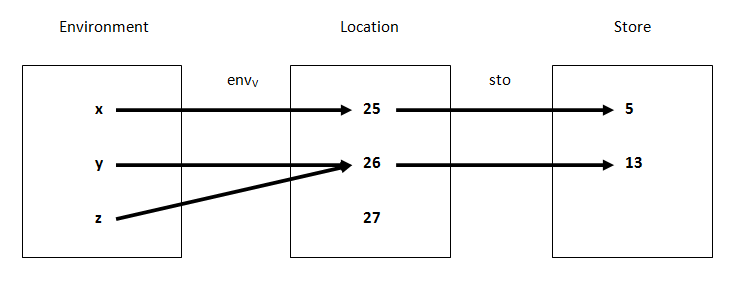
\includegraphics{billeder/environment_store_model.png}
\caption{Environment-store model}
\label{fig:esmodel}
\end{figure}


\section{The scope rules}\label{sec:scope-rules}



\todo{Matti: Er der en som kan forklare denne? Eller en som ved hvad den betyder som vil tjekke om den er korrekt, eventuelt skrive en forklaring til.}
\begin{center}
\begin{tabular}{ l l}
\hline
& \\
$[CALL-STAT-STAT_{BSS}]$ & $env'_{v}~[next \rightarrow l], env'_{p}~ \vdash \langle S,sto \rangle \rightarrow sto' \over env_{v}, ~ env_{p} \vdash \langle call~p, sto \rangle \rightarrow sto'$ \\
& where $env_{p}p = (S,env'{v},env'{p})$ \\
& and $l = env_{v}next$ \\
\hline
\end{tabular}
\end{center}







